% presentaciones/sesion04-cap04/sesion04.tex
% Sesión 4 — Capítulo 4: Base tecnológica: buscadores, plataformas, redes y comercio electrónico
% Laboratorio: Gestión de datos, comportamiento y perfiles del consumidor digital
% Lic. en Mercadotecnia Digital · ESCA Unidad Santo Tomás · IPN
% Fuente de contenido: libro-consumidor-digital/partes/parte1/cap04.tex
% Figuras reutilizadas del libro (TikZ y MATLAB) sin copiarlas: ver \graphicspath y \input.
\documentclass[aspectratio=169,xcolor=dvipsnames]{beamer}
\usetheme{Berlin}

%----------------------------------------------------------------------------------------
%   PALETA INSTITUCIONAL IPN (Manual de Identidad Gráfica, Pantone 222C)
%----------------------------------------------------------------------------------------
\usepackage[dvipsnames,svgnames,x11names]{xcolor}
\definecolor{IPNguinda}{HTML}{6F1D46}       % Pantone 222C oficial — color primario
\definecolor{IPNguindaOsc}{HTML}{45102C}    % sombra / paleta secundaria
\definecolor{IPNguindaClara}{HTML}{F4E9EF}  % fondo de bloques normales
\definecolor{IPNdorado}{HTML}{B8975A}       % dorado — SOLO enlaces y detalles del cierre
\definecolor{IPNterracota}{HTML}{9C5B44}    % alertblock
\definecolor{IPNterracotaClara}{HTML}{F6ECE6}
\definecolor{IPNbronce}{HTML}{8C6B3F}       % exampleblock
\definecolor{IPNbronceClaro}{HTML}{F5F0E3}
\definecolor{IPNgris}{HTML}{58595B}         % texto secundario / notas

% Alias con los nombres de config/colores.tex del libro, para que las figuras
% TikZ del libro se puedan \input sin modificarlas
\colorlet{guindaIPN}{IPNguinda}
\colorlet{guindaIPNOsc}{IPNguindaOsc}
\colorlet{guindaIPNClara}{IPNguindaClara}
\colorlet{doradoIPN}{IPNdorado}
\colorlet{bronceIPN}{IPNbronce}
\colorlet{bronceIPNClaro}{IPNbronceClaro}
\colorlet{grisIPN}{IPNgris}
\colorlet{terracotaIPN}{IPNterracota}
\colorlet{terracotaIPNClara}{IPNterracotaClara}
\definecolor{colorLaboratorio}{HTML}{1B6E7A}

\setbeamercolor{palette primary}{bg=IPNguinda,fg=white}
\setbeamercolor{palette secondary}{bg=IPNguindaOsc,fg=white}
\setbeamercolor{palette tertiary}{bg=IPNguindaOsc,fg=white}
\setbeamercolor{palette quaternary}{bg=IPNguinda,fg=white}
\setbeamercolor{structure}{fg=IPNguinda}
\setbeamercolor{title}{bg=IPNguinda,fg=white}
\setbeamercolor{frametitle}{bg=IPNguinda,fg=white}
\setbeamercolor{block title}{bg=IPNguinda,fg=white}
\setbeamercolor{block body}{bg=IPNguindaClara,fg=black}
\setbeamercolor{block title alerted}{bg=IPNterracota,fg=white}
\setbeamercolor{block body alerted}{bg=IPNterracotaClara,fg=black}
\setbeamercolor{block title example}{bg=IPNbronce,fg=white}
\setbeamercolor{block body example}{bg=IPNbronceClaro,fg=black}
\setbeamercolor{alerted text}{fg=IPNterracota}
\setbeamercolor{item}{fg=IPNguinda}
\setbeamercolor{section in toc}{fg=IPNguinda}
\setbeamercolor{footline}{bg=IPNguindaOsc,fg=white}

\usepackage[spanish,es-noshorthands,es-nodecimaldot]{babel}
\usepackage{csquotes}
\usepackage{hyperref}
\usepackage{graphicx}
\usepackage{booktabs}
\usepackage{array}
\usepackage{amsmath}
\setbeamertemplate{caption}[numbered]
\usepackage{xurl}
\usepackage{adjustbox}
\usepackage{tikz}
\usetikzlibrary{arrows.meta,positioning}
\usepackage{pgfplots}
\pgfplotsset{compat=1.18}

\graphicspath{{Figures/}{../../libro-consumidor-digital/figuras/matlab/}}
\newcommand{\figtikz}[1]{../../libro-consumidor-digital/figuras/tikz/#1}
\newcommand{\fuente}[1]{{\tiny\color{IPNgris}Fuente: #1}}

\hypersetup{
    colorlinks=true,
    linkcolor=IPNdorado,
    filecolor=IPNguinda,
    urlcolor=IPNguinda,
    citecolor=IPNguinda,
    pdftitle={Sesion 4 - Base tecnologica del consumidor digital},
    pdfauthor={Dr. Aboud Barsekh-Onji},
}

%----------------------------------------------------------------------------------------
%   CODE LISTINGS — sintaxis ESTÁNDAR del lenguaje
%----------------------------------------------------------------------------------------
\usepackage{listings}
\definecolor{backcolour}{rgb}{0.97,0.97,0.99}
\definecolor{codegreen}{rgb}{0,0.6,0}

\lstdefinestyle{MATLABStyle}{
  language=Matlab,
  basicstyle=\ttfamily\scriptsize,
  keywordstyle=\color{blue}\bfseries,
  commentstyle=\color{codegreen},
  stringstyle=\color{violet},
  breaklines=true,
  numbers=left,
  numbersep=5pt,
  frame=lines,
  backgroundcolor=\color{backcolour}
}
\lstset{style=MATLABStyle}

%----------------------------------------------------------------------------------------
%   TITLE CONFIGURATION
%----------------------------------------------------------------------------------------
\logo{
\includegraphics[height=0.75cm]{ipn-escudo.png}}
\title[Sesión 4 · Base tecnológica]{Base tecnológica: buscadores, plataformas, redes y comercio electrónico}
\subtitle{Sesión 4 · Unidad I — Capítulo 4}
\author{Dr. Aboud Barsekh-Onji}
\institute[IPN]{
    Instituto Politécnico Nacional \\
    \small ESCA Unidad Santo Tomás · Lic. en Mercadotecnia Digital \\
    \footnotesize Laboratorio: Gestión de datos, comportamiento y perfiles del consumidor digital
}
\date{\today}

%----------------------------------------------------------------------------------------
%   AUTO AGENDA AT EACH SECTION
%----------------------------------------------------------------------------------------
\AtBeginSection[]{
  \begin{frame}{Agenda}
    \tableofcontents[currentsection]
  \end{frame}
}


\begin{document}

\begin{frame}
    \titlepage
    \vspace{-4pt}
    \begin{center}
        {\tiny\color{IPNgris} ORCID: \href{https://orcid.org/0009-0004-5440-8092}{0009-0004-5440-8092}}
    \end{center}
\end{frame}

%------------------------------------------------
\section{Encuadre}
%------------------------------------------------

\begin{frame}{Ficha de la sesión}
\begin{columns}[T]
  \column{0.52\textwidth}
  \begin{block}{Unidad I}
    \small Comportamiento, perfil y gestión de datos del consumidor digital
  \end{block}
  \begin{block}{Tema del programa (1.4 Base tecnológica)}
    \scriptsize
    \begin{itemize}
      \item[1.4.1] Temas selectos de buscadores y plataformas de gestión integral, redes sociales y comercio electrónico
    \end{itemize}
  \end{block}
  \column{0.44\textwidth}
  \begin{block}{Carga horaria}
    \small Teoría 3.0 h · Práctica 2.0 h\\ Aprendizaje autónomo 1.0 h
  \end{block}
  \begin{exampleblock}{Competencia de la unidad}
    \small Identifica el comportamiento del consumidor digital y su evolución a partir de sus tipos de perfil y gestión de datos.
  \end{exampleblock}
\end{columns}
\end{frame}

\begin{frame}{Al terminar la sesión podrás\ldots}
\begin{enumerate}
  \item \textbf{Aplicar} una matriz de criterios durables para evaluar cualquier plataforma digital, presente o futura.
  \vspace{6pt}
  \item \textbf{Interpretar} una serie de interés de búsqueda separando su tendencia, su estacionalidad y su ruido.
  \vspace{6pt}
  \item \textbf{Extraer} y analizar la frecuencia de términos de un conjunto de comentarios de escucha social.
\end{enumerate}
\vspace{8pt}
\begin{alertblock}{Recordatorio}
  Aprendizaje autónomo de la Sesión 3: entrega a más tardar el \textbf{jueves 15 de octubre}, en su carpeta del portafolio.
\end{alertblock}
\end{frame}

\begin{frame}{Arranque: ¿qué plataforma cambió en tu vida digital?}
\begin{columns}[T]
  \column{0.55\textwidth}
  \begin{exampleblock}{Pregunta de arranque}
    Piensen en una red social, un buscador o una tienda en línea que \textbf{usaban hace tres años} y que hoy usan distinto (o ya no usan).\\[4pt]
    ¿Qué cambió: la plataforma, ustedes, o ambas? ¿Qué pasaría si la plataforma desapareciera mañana?
  \end{exampleblock}
  \vspace{4pt}
  {\small\color{IPNgris} Puente con la Sesión 3: la base legal y los datos de primera parte.}
  \column{0.41\textwidth}
  \begin{block}{Dinámica (10 min)}
    \small
    \begin{enumerate}
      \item Individual: anoten la plataforma y qué \enquote{les daba} (2 min).
      \item Parejas: ¿qué dato suyo se llevaba esa plataforma?
      \item Pizarrón: lista de plataformas \textbf{que ya no existen o cambiaron}. Vuelve en la matriz de criterios.
    \end{enumerate}
  \end{block}
\end{columns}
\end{frame}

%------------------------------------------------
\section[Apertura]{Caso de apertura}
%------------------------------------------------

\begin{frame}{Dos predicciones razonables que no se cumplieron}
\begin{columns}[T]
  \column{0.48\textwidth}
  \begin{block}{Cookies de terceros (2020--2023)}
    \small La industria advertía que desaparecerían de Chrome en dos o tres años.\\[3pt]
    \textbf{A sept. 2026:} siguen activas por defecto; Google revirtió el plan.
  \end{block}
  \column{0.48\textwidth}
  \begin{block}{Búsqueda tradicional (Gartner, 2024)}
    \small Predijo una caída de \textbf{25\,\%} del volumen para 2026 por los chatbots de IA.\\[3pt]
    \textbf{A sept. 2026:} las fuentes de industria se contradicen sobre si ocurrió.
  \end{block}
\end{columns}
\vspace{6pt}
\begin{alertblock}{La premisa incómoda del capítulo}
  Cualquier cifra puntual de cuota de mercado o de adopción tecnológica puede estar \textbf{desactualizada antes de que egresen}. Por eso no aprendemos un catálogo de plataformas: aprendemos \textbf{criterios para evaluar cualquiera}.
\end{alertblock}
\end{frame}

%------------------------------------------------
\section[Criterios]{1.4.1 Matriz de criterios durables}
%------------------------------------------------

\begin{frame}{Cuatro criterios que sobreviven al cambio de marcas}
\begin{center}
  \resizebox{!}{0.40\textheight}{\input{\figtikz{cap04-criterios-evaluacion}}}
\end{center}
\vspace{2pt}
\begin{itemize}
  \small
  \item El programa deja el subtema abierto (\enquote{temas selectos}) porque el panorama cambia más rápido que un libro.
  \item Se aplican a \textbf{buscadores, plataformas, redes sociales y comercio electrónico} por igual.
\end{itemize}
\fuente{elaboración propia.}
\end{frame}

\begin{frame}{La pregunta que se hace con cada criterio}
\footnotesize
\begin{center}
\begin{tabular}{@{}>{\raggedright}p{2.7cm}>{\raggedright\arraybackslash}p{9.6cm}@{}}
\toprule
\textbf{Criterio} & \textbf{Pregunta de evaluación} \\
\midrule
Modelo de negocio & ¿Se financia por publicidad, suscripción o comisión transaccional? Cada modelo alinea sus incentivos de forma distinta con los del consumidor. \\
Intermediación de datos & ¿Quién es dueño del dato de comportamiento: la organización que anuncia, la plataforma, o ambas bajo condiciones específicas? \\
Interoperabilidad & ¿Ofrece APIs abiertas para exportar datos propios, o los mantiene cautivos en su ecosistema cerrado? \\
Exposición regulatoria & ¿Qué marco aplica (DSA europea, LFPDPPP mexicana, ninguno vigente todavía) y qué riesgo de cumplimiento implica usarla? \\
\bottomrule
\end{tabular}
\end{center}
\fuente{elaboración propia.}
\end{frame}

\begin{frame}{Dinámica: apliquen la matriz (8 min)}
\begin{columns}[T]
  \column{0.52\textwidth}
  \begin{exampleblock}{En parejas}
    \small Elijan \textbf{una plataforma que usen a diario} y respondan una pregunta por criterio:
    \begin{enumerate}
      \scriptsize
      \item ¿Cómo gana dinero con ustedes?
      \item ¿Qué dato suyo genera y quién lo controla?
      \item ¿Pueden llevarse sus datos a otra plataforma?
      \item ¿Qué ley o guía le aplica en México?
    \end{enumerate}
  \end{exampleblock}
  \column{0.44\textwidth}
  \begin{alertblock}{Pista}
    \small Si no encuentran la respuesta a un criterio, \textbf{eso ya es un hallazgo}: la plataforma no lo hace transparente.
  \end{alertblock}
  {\small\color{IPNgris} Insumo del reporte de indagación documental del portafolio.}
\end{columns}
\end{frame}

\begin{frame}{Frontera: el comercio agéntico como capa de intermediación}
\begin{center}
  \resizebox{0.78\linewidth}{!}{\input{\figtikz{cap04-comercio-agentico}}}
\end{center}
\vspace{2pt}
\begin{itemize}
  \scriptsize
  \item \textbf{Comercio agéntico:} asistentes de compra basados en IA que buscan, comparan y a veces ejecutan la compra por el consumidor.
  \item Según el libro (a sept. 2026) conviven dos protocolos abiertos en competencia (Agentic Commerce Protocol, de Stripe y OpenAI; Universal Commerce Protocol, de Google) y el enfoque propietario de Amazon (Rufus, Alexa+).
  \item \textbf{La pregunta durable no es qué asistente tiene más usuarios}, sino \textbf{quién controla la capa de intermediación} entre consumidor y punto de venta.
\end{itemize}
\fuente{elaboración propia con base en Kotler et al. (2024) y Mathur et al. (2019). Verifica el estado vigente: cambia rápido.}
\end{frame}

\begin{frame}{La intermediación puede sesgar la decisión}
\begin{columns}[T]
  \column{0.52\textwidth}
  \begin{block}{Patrones oscuros (Mathur et al., 2019)}
    \small Taxonomía empírica de patrones oscuros en 11{,}000 sitios de comercio electrónico: \textbf{cualquier capa con suficiente control sobre la interfaz} puede, sin cambiar de tecnología, \textbf{pasar de facilitar la decisión a sesgarla}.
  \end{block}
  \column{0.44\textwidth}
  \begin{alertblock}{Aplicado a la matriz}
    \small Un asistente de compra con incentivos de \textbf{comisión} (criterio 1) y control del dato (criterio 2) puede favorecer a quien le paga más, no a quien mejor sirve al consumidor.
  \end{alertblock}
\end{columns}
\vspace{6pt}
{\small\color{IPNgris} Se desarrolla con detalle en el Capítulo 7.}
\end{frame}

\begin{frame}{Redes sociales y comercio electrónico: tres criterios extra}
\begin{columns}[T]
  \column{0.31\textwidth}
  \begin{block}{Cobertura omnicanal}
    \small ¿Comparte una identidad única entre canales? (Verhoef et al., 2015; Sesión 3.)
  \end{block}
  \column{0.31\textwidth}
  \begin{exampleblock}{Atribución multi-touch}
    \small ¿Se puede rastrear \textbf{qué canal contribuyó} a una conversión, no solo el último clic?
  \end{exampleblock}
  \column{0.31\textwidth}
  \begin{block}{Exposición regulatoria}
    \small LFPDPPP y la Guía de Publicidad para Influencers de PROFECO.
  \end{block}
\end{columns}
\vspace{6pt}
\begin{alertblock}{Ojo con la Guía de PROFECO}
  \small Es una \textbf{guía de recomendaciones} con fundamento en la Ley Federal de Protección al Consumidor (DOF, agosto de 2023), \textbf{no} una ley específica con régimen sancionador propio.
\end{alertblock}
\end{frame}

%------------------------------------------------
\section[Evidencia]{Evidencia: predicciones y datos}
%------------------------------------------------

\begin{frame}{Predicciones frente a lo verificable}
\footnotesize
\begin{center}
\begin{tabular}{@{}>{\raggedright}p{3.1cm}>{\raggedright}p{3.4cm}>{\raggedright\arraybackslash}p{4.6cm}@{}}
\toprule
\textbf{Predicción} & \textbf{Lo anunciado} & \textbf{Lo verificable a sept. 2026} \\
\midrule
Fin de cookies de terceros en Chrome (industria, 2020--2023) & Desaparición completa \enquote{en 2024} o \enquote{en 2025} & Siguen activas por defecto; Google revirtió el plan \\
Caída del volumen de búsqueda tradicional (Gartner, 2024) & $-$25\,\% para 2026 por chatbots de IA & Las fuentes de industria se contradicen entre sí \\
\bottomrule
\end{tabular}
\end{center}
\vspace{2pt}
\begin{alertblock}{No es una crítica a Gartner}
  \scriptsize Ambas predicciones fueron razonables y de fuentes de jerarquía comparable. Es una \textbf{demostración metodológica}: quien memoriza la predicción en vez del criterio queda desactualizado antes de graduarse.
\end{alertblock}
\fuente{elaboración propia con base en European Parliamentary Research Service (2025) y la investigación documental del libro.}
\end{frame}

\begin{frame}{Por qué el libro no da cifras de cuota de mercado}
\begin{columns}[T]
  \column{0.52\textwidth}
  \begin{block}{Lo que se encontró}
    \small Toda cifra puntual de adopción (cuota de buscadores, tráfico impulsado por IA generativa, tamaño del comercio agéntico) provenía de \textbf{blogs de industria o predicciones de analistas}, no de fuentes primarias verificables.
  \end{block}
  \column{0.44\textwidth}
  \begin{exampleblock}{Criterio de verificación}
    \small Lo que no se puede confirmar en fuente primaria \textbf{no se reporta como dato duro}. Esa decisión es, en sí misma, \textbf{la evidencia más honesta} del capítulo.
  \end{exampleblock}
\end{columns}
\vspace{6pt}
\begin{center}\small Desconfiar de una cifra sin metodología pública es una \textbf{competencia profesional}.\end{center}
\end{frame}

%------------------------------------------------
\section[Laboratorio]{Laboratorio MATLAB}
%------------------------------------------------

\begin{frame}{Laboratorio: tendencia, estacionalidad y texto}
\begin{block}{Objetivo}
  Descomponer una serie de interés de búsqueda y extraer la frecuencia de términos de comentarios de escucha social: los dos tipos de dato que alimentan el análisis de la base tecnológica.
\end{block}
\begin{columns}[T]
  \column{0.48\textwidth}
  \begin{exampleblock}{Serie de tiempo}
    \small
    \[ y_t = T_t + S_t + \varepsilon_t \]
    \scriptsize
    $T_t$ tendencia (largo plazo), $S_t$ estacionalidad (se repite cada año), $\varepsilon_t$ ruido.
  \end{exampleblock}
  \column{0.48\textwidth}
  \begin{block}{Bolsa de palabras}
    \scriptsize Cada comentario se separa en palabras, se quitan las \textbf{palabras vacías} (el, la, de\ldots) y se \textbf{cuenta cuántas veces aparece} cada término en todo el conjunto.
  \end{block}
\end{columns}
\end{frame}

\begin{frame}{Cómo se separa la tendencia de la temporada}
\begin{columns}[T]
  \column{0.56\textwidth}
  \begin{block}{Promedio móvil de 52 semanas}
    \small En cada semana se promedian las 52 semanas alrededor. Como abarca \textbf{un año completo}, el efecto de la temporada \textbf{se cancela} y queda la tendencia.
  \end{block}
  \begin{exampleblock}{Estacionalidad}
    \small Es lo que sobra: \textbf{serie $-$ tendencia}.
  \end{exampleblock}
  \column{0.40\textwidth}
  \begin{alertblock}{Dos advertencias}
    \scriptsize
    \begin{itemize}
      \item Si el promedio abarca \textbf{menos de un ciclo}, la tendencia se \enquote{come} parte de la temporada.
      \item En los \textbf{extremos} de la serie el promedio es incompleto: ahí la estimación es menos confiable.
    \end{itemize}
  \end{alertblock}
\end{columns}
\end{frame}

\begin{frame}[fragile]{El script: \texttt{cap04\_series\_texto.m}}
\begin{columns}[T]
  \column{0.60\textwidth}
\begin{lstlisting}[basicstyle=\ttfamily\scriptsize]
%% ==================================
%  PARAMETROS: UNICA SECCION QUE
%  EL ESTUDIANTE DEBE EDITAR
%  ==================================
nSemanas = 104;      % duracion (semanas)
fechaInicio = datetime(2024,9,16);
crecimientoSemanal = 0.35; % tendencia
amplitudEstacional = 12;   % pico anual
desviacionRuido = 4;       % ruido
\end{lstlisting}
  \column{0.36\textwidth}
  \begin{block}{Reglas y rangos}
    \scriptsize
    \begin{itemize}
      \item Amplitud y ruido: valores reales $\geq 0$ (0 = sin estacionalidad / sin ruido).
      \item Crecimiento: positivo sube, negativo baja, 0 plana.
      \item Datos \textbf{sintéticos} (\texttt{rng(42)}); el corpus de 20 comentarios es fijo.
    \end{itemize}
  \end{block}
  \begin{exampleblock}{Sin MATLAB}
    \scriptsize \texttt{cap04\_series\_texto\_\allowbreak interactivo.html}: mismos parámetros y casos A, B, C.
  \end{exampleblock}
\end{columns}
\end{frame}

\begin{frame}{Salida: serie, tendencia y estacionalidad}
\begin{center}
  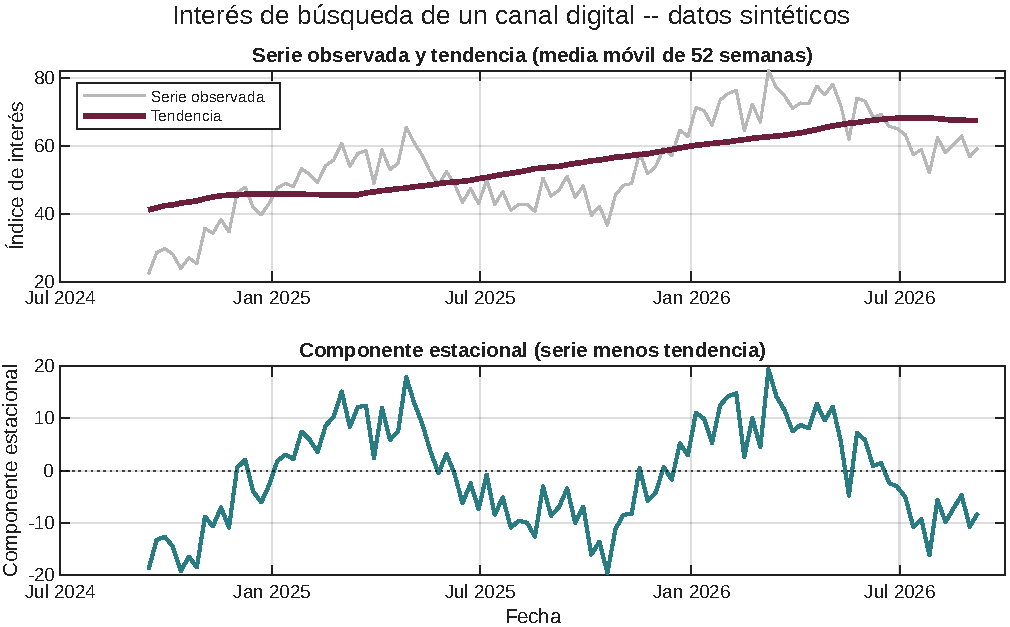
\includegraphics[width=\linewidth,height=0.62\textheight,keepaspectratio]{cap04_tendencia_estacionalidad.pdf}
\end{center}
\vspace{-4pt}
\begin{center}
  \small Amplitud estacional estimada: \textbf{38.9 puntos} · máximo de la serie: \textbf{82.0}
\end{center}
\fuente{elaboración propia, MATLAB, datos sintéticos, \texttt{rng(42)}.}
\end{frame}

\begin{frame}{Interpretación de negocio}
\begin{columns}[c]
  \column{0.48\textwidth}
  \begin{block}{Lo que la serie oculta}
    \small En el panel superior (gris) el ruido tapa un \textbf{pico recurrente} que sí aparece en el panel inferior: en esta serie sintética, hacia \textbf{marzo-abril} de cada ciclo y de magnitud similar en los dos años.
  \end{block}
  \begin{alertblock}{El error costoso}
    \small Planear inventario, personal o publicidad sin aislar la estacionalidad es leer como \enquote{tendencia acelerada} lo que es la \textbf{fase ascendente, predecible,} del ciclo.
  \end{alertblock}
  \column{0.48\textwidth}
  \begin{exampleblock}{Cuidado con los extremos}
    \small Los primeros y últimos meses usan un promedio incompleto: la estacionalidad ahí \textbf{se infla}. Confirmen con más de dos ciclos antes de decidir inversiones.
  \end{exampleblock}
\end{columns}
\end{frame}

\begin{frame}{Salida: nube de palabras de escucha social}
\begin{columns}[c]
  \column{0.52\textwidth}
  \centering
  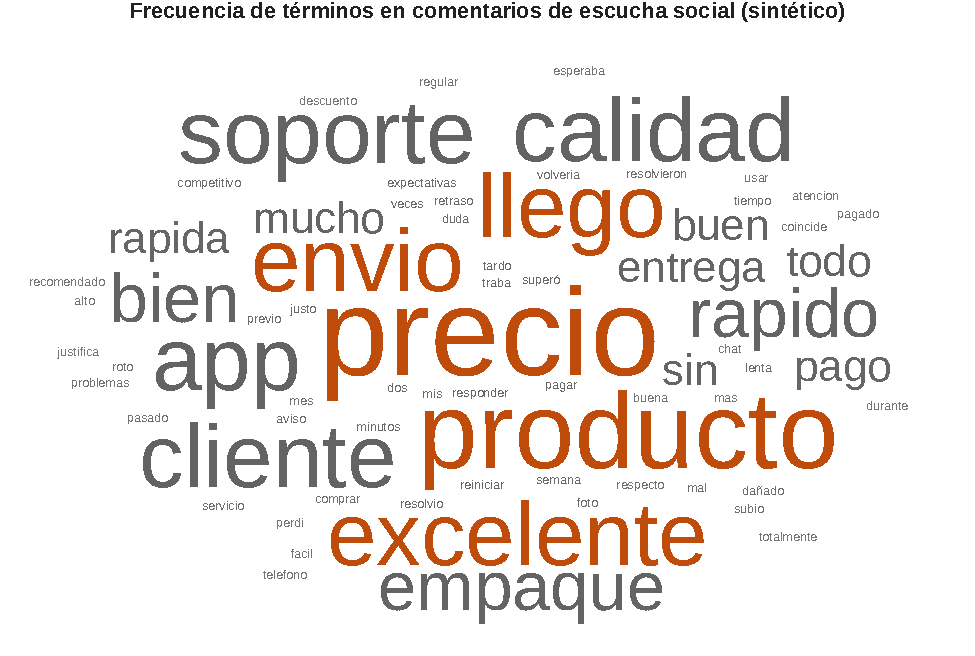
\includegraphics[width=\linewidth,height=0.62\textheight,keepaspectratio]{cap04_nube_palabras.pdf}
  \column{0.44\textwidth}
  \begin{block}{Lo que se ve}
    \small Dominan \textit{precio}, \textit{producto}, \textit{envío}, \textit{llegó}, \textit{excelente} y \textit{soporte}.
  \end{block}
  \begin{alertblock}{Lo que no se ve}
    \small Mezclan menciones \textbf{positivas} y \textbf{de fricción} que, por tamaño, \textbf{no se distinguen}. Hay que clasificarlas a mano.
  \end{alertblock}
\end{columns}
\fuente{elaboración propia, corpus sintético de 20 comentarios.}
\end{frame}

\begin{frame}{Ejercicio propuesto: tres corridas}
\begin{columns}[T]
  \column{0.48\textwidth}
  \begin{exampleblock}{Casos (solo el bloque de parámetros)}
    \scriptsize
    \begin{itemize}
      \item[\textbf{A}] Valores por defecto.
      \item[\textbf{B}] \textbf{Estacionalidad débil}: \texttt{amplitudEstacional} de 12 a 3.
      \item[\textbf{C}] \textbf{Más ruido}: \texttt{amplitudEstacional} en 12 y \texttt{desviacionRuido} de 4 a 15.
    \end{itemize}
  \end{exampleblock}
  \column{0.48\textwidth}
  \footnotesize
  \begin{tabular}{@{}lcc@{}}
    \toprule
    Caso & Amplitud estimada & Máximo de la serie \\
    \midrule
    A & \rule{1.3cm}{0.4pt} & \rule{1.3cm}{0.4pt} \\[2pt]
    B & \rule{1.3cm}{0.4pt} & \rule{1.3cm}{0.4pt} \\[2pt]
    C & \rule{1.3cm}{0.4pt} & \rule{1.3cm}{0.4pt} \\
    \bottomrule
  \end{tabular}
\end{columns}
\vspace{2pt}
\begin{block}{Respondan con sus corridas}
  \scriptsize
  \begin{enumerate}
    \item Caso B: ¿el componente estacional sigue siendo visible \textbf{a simple vista} en la serie observada?
    \item Caso C: ¿la tendencia sigue viéndose suave o el ruido empieza a distorsionarla?
    \item ¿Cuándo es más fácil \textbf{confundir estacionalidad con tendencia}: poco ruido y estacionalidad marcada, o mucho ruido y estacionalidad débil?
  \end{enumerate}
\end{block}
\end{frame}

\begin{frame}{Segunda parte: clasifiquen los 10 términos más frecuentes}
\begin{columns}[T]
  \column{0.50\textwidth}
  \begin{block}{A mano, en tres categorías}
    \small
    \begin{itemize}
      \item \textbf{Experiencia positiva}
      \item \textbf{Fricción operativa}
      \item \textbf{Neutro / descriptivo}
    \end{itemize}
  \end{block}
  \column{0.46\textwidth}
  \begin{alertblock}{Para discutir}
    \small Sin ese trabajo manual, ¿la nube de palabras es una \textbf{herramienta de análisis} o solo de \textbf{exploración inicial}?
  \end{alertblock}
\end{columns}
\vspace{6pt}
\begin{center}\small \textit{precio} puede ser positivo (\enquote{precio justo}) o fricción (\enquote{el precio subió mucho}): la palabra sola no dice cuál.\end{center}
\end{frame}

\begin{frame}{Práctica con sus propios datos: app HTML}
\begin{columns}[T]
  \column{0.54\textwidth}
  \begin{block}{\texttt{cap04\_series\_datos\_propios.html}}
    \small Sin MATLAB y sin conexión: suban un Excel con \textbf{una serie de tiempo} (y, si quieren, comentarios) y recorran cinco pasos:
    \scriptsize
    \begin{enumerate}
      \item Calidad de la serie (faltantes, intervalos).
      \item Tendencia y estacionalidad, con el perfil por mes.
      \item \textbf{¿Campaña o temporada?}: último año contra el año anterior.
      \item Escucha social: nube, frecuencia y clasificación manual.
      \item Lectura de negocio y descarga en Excel.
    \end{enumerate}
  \end{block}
  \column{0.42\textwidth}
  \begin{exampleblock}{Reglas del archivo}
    \scriptsize
    \begin{itemize}
      \item Hoja \texttt{Serie}: \texttt{Fecha} y un valor, una fila por semana, mes o día.
      \item Hoja \texttt{Comentarios} (opcional): un comentario por fila.
      \item \textbf{Sin} nombres de usuario ni datos que identifiquen personas.
      \item Sus datos \textbf{no salen} de su computadora.
    \end{itemize}
  \end{exampleblock}
\end{columns}
\end{frame}

\begin{frame}{Ética: la escucha social no está exenta de la ley}
\begin{alertblock}{Publicar una opinión no es dar consentimiento ilimitado}
  Un corpus real de escucha social contiene texto de personas \textbf{identificables o potencialmente identificables}. Analizarlo, incluso de forma agregada, implica las mismas obligaciones de \textbf{base legal} de la Sesión 3.
\end{alertblock}
\begin{block}{Como mínimo}
  \begin{itemize}
    \item Que los comentarios sean públicos \textbf{no basta} para justificar cualquier uso analítico posterior.
    \item Verificar la \textbf{LFPDPPP vigente} al implementar, no solo al estudiar.
  \end{itemize}
\end{block}
\end{frame}

%------------------------------------------------
\section[Caso]{Estudio de caso}
%------------------------------------------------

\begin{frame}{Caso: la marca de electrodomésticos}
\begin{exampleblock}{Caso ficticio}
  El equipo de mercadotecnia observa que su índice de interés de búsqueda de marca \textbf{subió 20 puntos} en las últimas cuatro semanas y concluye que la campaña reciente de \textit{influencer marketing} funciona muy bien. Quiere \textbf{duplicar el presupuesto} de inmediato.
\end{exampleblock}
\begin{alertblock}{Lo que descubre el analista}
  \small Al revisar \textbf{dos años} de la serie (no solo cuatro semanas), el mismo salto de unos 20 puntos ocurrió \textbf{en la misma época del año anterior}, sin ninguna campaña de influencers.
\end{alertblock}
\end{frame}

\begin{frame}{El caso en una gráfica (datos sintéticos)}
\begin{center}
\begin{tikzpicture}
  \begin{axis}[
      width=0.92\linewidth, height=4.4cm, xmin=1, xmax=104, ymin=0, ymax=100,
      xlabel={semana (1 = 7-oct-2024)}, ylabel={índice de interés},
      label style={font=\scriptsize}, tick label style={font=\scriptsize},
      axis lines*=left, ymajorgrids, grid style={IPNgris!25},
    ]
    \fill[IPNdorado!35] (axis cs:49,0) rectangle (axis cs:52,100);
    \fill[IPNdorado!35] (axis cs:101,0) rectangle (axis cs:104,100);
    \addplot[IPNguinda, thick] coordinates {(1,69.3) (2,71.3) (3,77.2) (4,82.9) (5,80.2) (6,82.3) (7,89.3) (8,87.8) (9,84.5) (10,87.3) (11,83.5) (12,82.2) (13,82.4) (14,73.6) (15,71.3) (16,71.4) (17,66.4) (18,66.3) (19,58.4) (20,52.3) (21,56.3) (22,46.5) (23,42.7) (24,33.6) (25,31.7) (26,29.3) (27,21.5) (28,22.4) (29,16.2) (30,14.2) (31,10.9) (32,16.4) (33,9.4) (34,5.5) (35,11.0) (36,5.2) (37,10.5) (38,5.5) (39,9.5) (40,16.7) (41,21.4) (42,23.2) (43,26.2) (44,29.9) (45,30.9) (46,37.9) (47,43.5) (48,53.0) (49,55.8) (50,54.3) (51,65.3) (52,67.6) (53,71.0) (54,78.8) (55,83.5) (56,86.3) (57,83.6) (58,87.3) (59,90.7) (60,93.6) (61,89.7) (62,90.4) (63,86.8) (64,85.2) (65,89.4) (66,88.6) (67,81.4) (68,81.3) (69,75.7) (70,68.7) (71,67.4) (72,66.4) (73,57.0) (74,57.1) (75,39.8) (76,45.5) (77,38.8) (78,33.3) (79,30.5) (80,20.5) (81,22.5) (82,21.4) (83,22.3) (84,14.4) (85,12.2) (86,12.4) (87,16.4) (88,15.1) (89,13.5) (90,18.1) (91,19.0) (92,24.2) (93,22.3) (94,26.9) (95,30.6) (96,31.6) (97,41.4) (98,46.0) (99,50.1) (100,54.3) (101,55.7) (102,63.5) (103,68.5) (104,71.6)};
    \node[font=\tiny, text=IPNbronce] at (axis cs:50.5,94) {hace 1 año};
    \node[font=\tiny, text=IPNbronce] at (axis cs:99.5,94) {últimas 4};
  \end{axis}
\end{tikzpicture}
\end{center}
\vspace{-2pt}
\begin{center}\scriptsize El salto aparece \textbf{dos veces}: en septiembre de 2025 y en septiembre de 2026. Es la firma de la \textbf{estacionalidad}, no de la campaña.\end{center}
\fuente{elaboración propia con datos sintéticos (Ejemplo 2 de la app).}
\end{frame}

\begin{frame}{Preguntas guía}
\small
\begin{enumerate}
  \item ¿Qué componente de la serie de tiempo (\textbf{tendencia o estacionalidad}) explica mejor el patrón que encontró el analista?
  \vspace{3pt}
  \item Diseñen, en términos generales, cómo el equipo podría \textbf{aislar el efecto real de la campaña} del efecto estacional con el enfoque de descomposición del laboratorio.
  \vspace{3pt}
  \item ¿Qué consecuencia de negocio tendría \textbf{duplicar el presupuesto} basándose en esa lectura?
  \vspace{3pt}
  \item Relacionen el caso con la advertencia del caso de apertura: ¿qué tienen en común el error de Gartner con el 25\,\% y el error del equipo de mercadotecnia?
\end{enumerate}
\begin{alertblock}{Entregable}
  \small Solución escrita con las cuatro preguntas respondidas.
\end{alertblock}
\end{frame}

%------------------------------------------------
\section{Cierre}
%------------------------------------------------

\begin{frame}{Síntesis: criterios, no catálogos}
\begin{itemize}
  \small
  \item La base tecnológica cambia más rápido de lo que un libro (o una investigación) puede verificar: \textbf{se dominan criterios, no marcas}.
  \item Cuatro criterios durables: \textbf{modelo de negocio, intermediación de datos, interoperabilidad y exposición regulatoria}; en redes y comercio, además omnicanalidad y atribución.
  \item Dos herramientas analíticas: \textbf{separar tendencia de estacionalidad} en una serie y \textbf{contar términos} en un corpus de texto.
  \item Una nube de palabras \textbf{explora}; no interpreta. Y la escucha social \textbf{requiere base legal}.
\end{itemize}
\vspace{4pt}
\begin{alertblock}{La regla de la sesión}
  \small Antes de atribuirle un salto a la campaña, pregunten: \textbf{¿pasó lo mismo en esta época el año pasado?}
\end{alertblock}
\end{frame}

\begin{frame}{Autoevaluación rápida}
\footnotesize
\begin{enumerate}
  \item El capítulo propone una matriz de criterios en vez de un catálogo de herramientas porque:
  \begin{itemize}
    \item[a)] las herramientas actuales son de mala calidad;
    \item[b)] \alt<2->{\textcolor{IPNguinda}{\textbf{un catálogo de marcas envejece más rápido que los criterios que las evalúan}}}{un catálogo de marcas envejece más rápido que los criterios que las evalúan};
    \item[c)] el programa oficial prohíbe mencionar marcas.
  \end{itemize}
  \item En el laboratorio, el componente estacional se obtiene como:
  \begin{itemize}
    \item[a)] la serie observada multiplicada por dos;
    \item[b)] \alt<2->{\textcolor{IPNguinda}{\textbf{la serie observada menos la tendencia estimada}}}{la serie observada menos la tendencia estimada};
    \item[c)] el promedio simple de toda la serie.
  \end{itemize}
  \item Una nube de palabras, por sí sola, es:
  \begin{itemize}
    \item[a)] un análisis completo del sentimiento de los clientes;
    \item[b)] \alt<2->{\textcolor{IPNguinda}{\textbf{una herramienta de exploración inicial: no distingue si un término es positivo o de fricción}}}{una herramienta de exploración inicial: no distingue si un término es positivo o de fricción};
    \item[c)] una prueba de que la campaña funcionó.
  \end{itemize}
\end{enumerate}
\end{frame}

\begin{frame}{Evidencias del portafolio}
\begin{block}{Pasos para subir los trabajos al portafolio}
    \begin{itemize}
    \item Accede a esta carpeta de evidencia: \url{https://drive.google.com/drive/folders/1sr_SAVkl_Mjil6ZRWz3O2mveMoZVW6cp?usp=sharing}
    \item Crea una carpeta con tu nombre y organiza en ella todos tus entregables del semestre.
    \item Considera los tiempos límite establecidos para cada actividad.
    \end{itemize}
  \end{block}
\end{frame}

\begin{frame}{Evidencias del portafolio}
\small
\begin{columns}[T]
  \column{0.48\textwidth}
  \begin{block}{Reporte de indagación documental}
    \scriptsize Aplicar la matriz de cuatro criterios a \textbf{dos plataformas digitales vigentes} elegidas por el equipo, con al menos una fuente por criterio.
  \end{block}
  \begin{block}{Exposición}
    \scriptsize Presentar el hallazgo del componente estacional del laboratorio y proponer una decisión de negocio distinta según se ignore o se considere.
  \end{block}
  \begin{block}{Solución de casos}
    \scriptsize Caso de la marca de electrodomésticos, cuatro preguntas por escrito.
  \end{block}
  \column{0.48\textwidth}
  \begin{block}{Reporte de práctica}
    \scriptsize Entregable único de la práctica \enquote{Buscadores y plataformas en la gestión de datos del consumidor digital}, junto con el reporte del Cap.~3, con el cuadro de los casos A, B y C.
  \end{block}
\end{columns}
\end{frame}

\begin{frame}{Aprendizaje autónomo}
\footnotesize
\begin{enumerate}
  \item Investigar, \textbf{con fecha de consulta registrada}, si el estado del comercio agéntico descrito en la sesión cambió de forma relevante desde el cierre del libro (18 de septiembre de 2026) y documentar la fuente.
  \vspace{1pt}
  \item Completar el \textbf{Caso C} en \texttt{cap04\_series\_texto\_\allowbreak interactivo.html} y anotar qué le pasa a la tendencia con más ruido.
  \vspace{1pt}
  \item Con \texttt{cap04\_series\_datos\_propios.html}, probar el \textbf{Ejemplo 2} y escribir en dos líneas por qué el salto es de temporada.
\end{enumerate}
\vspace{2pt}
\begin{alertblock}{Fecha de entrega}
  \textbf{Viernes 23 de octubre}, en su carpeta del portafolio.
\end{alertblock}
\end{frame}

\begin{frame}{Glosario de la sesión}
\scriptsize
\begin{description}
  \item[Matriz de criterios durables] Modelo de negocio, intermediación de datos, interoperabilidad y exposición regulatoria: sirven para evaluar cualquier plataforma.
  \item[Comercio agéntico] Compra mediada por asistentes de IA que buscan, comparan y a veces ejecutan la transacción por el consumidor.
  \item[Tendencia] Cambio de largo plazo de una serie, sin temporada ni ruido.
  \item[Estacionalidad] Patrón que se repite con periodo fijo (p.\,ej., anual). Se estima como serie $-$ tendencia.
  \item[Amplitud estacional] Qué tan marcado es el pico anual; $\geq 0$ (con 0 no hay estacionalidad).
  \item[Desviación del ruido] Dispersión aleatoria semana a semana; $\geq 0$.
  \item[Bolsa de palabras] Corpus de texto como tabla de frecuencias de términos por documento.
\end{description}
\end{frame}

\begin{frame}{Referencias}
\tiny
\begin{itemize}
  \item[] European Parliamentary Research Service. (2025). \textit{Regulating dark patterns in the EU: Towards digital fairness}. European Parliament.
  \item[] Diario Oficial de la Federación. (2025, 20 de marzo). \textit{Decreto por el que se expide la Ley Federal de Protección de Datos Personales en Posesión de los Particulares}. \url{https://www.diputados.gob.mx/LeyesBiblio/pdf/LFPDPPP.pdf}
  \item[] Kotler, P., Kartajaya, H. y Setiawan, I. (2024). \textit{Marketing 6.0: The future is immersive}. Wiley.
  \item[] Mathur, A., Acar, G., Friedman, M. J., Lucherini, E., Mayer, J., Chetty, M. y Narayanan, A. (2019). Dark patterns at scale: Findings from a crawl of 11K shopping websites. \textit{Proceedings of the ACM on Human-Computer Interaction, 3}(CSCW), 1--32. \url{https://doi.org/10.1145/3359183}
  \item[] Procuraduría Federal del Consumidor. (2023). \textit{Guía de Publicidad para Influencers}. Diario Oficial de la Federación. \url{https://dof.gob.mx/2023/PROFECO/guiainfluencers.pdf}
  \item[] Sheth, J. N. y Jain, V. (2026). \textit{Digital consumer behavior}. Routledge.
  \item[] Verhoef, P. C., Kannan, P. K. y Inman, J. J. (2015). From multi-channel retailing to omni-channel retailing. \textit{Journal of Retailing, 91}(2), 174--181. \url{https://doi.org/10.1016/j.jretai.2015.02.005}
\end{itemize}
\end{frame}

\begin{frame}
    \begin{center}
        {\Large \textcolor{IPNguinda}{\textbf{Gracias}}}\\[6pt]
        {\color{IPNdorado}\rule{0.4\linewidth}{1.2pt}}\\[6pt]
        Dr. Aboud Barsekh-Onji \\
        \small Instituto Politécnico Nacional · ESCA Unidad Santo Tomás \\
        \small \texttt{ORCID: \href{https://orcid.org/0009-0004-5440-8092}{0009-0004-5440-8092}}
    \end{center}
\end{frame}

\end{document}
